\chapter{Luna-Lander}\label{sec:LunaLander}
TODO (Begründen warum noch ein environment)

\section{Die Umgebung und die Aufgabe}
Wir nutzen für die folgenden Experimente das Toolkit \textit{OpenAi Gym} \cite{x03_openaiGym}. OpenAi Gym ist eine Kollektion von Environments, die für das Trainieren und Vergleichen von diversen Machine-Learning-Algorithmen gedacht sind. Die Entwickler wollen erreichen, die Umgebungen so zugänglich wie möglich zu machen.

Wir verwenden für unsere Versuche das Environment \glqq LunarLander-v2\grqq{}. Der Agent soll hierbei lernen, eine kleine, zweidimensionale Raumkapsel auf einer Landeplattform (markiert mit gelben Fahnen) zu landen. Hierbei ist es wichtig, dass das Raumschiff sachte auf dem Boden aufsetzt, ohne dass seine Landefüße beschädigt werden. Eine visuelle Repräsentation des Environments ist in Abbildung \ref{img:lunarLanderExample} dargestellt.

\begin{figure}[h!]
    \centering
    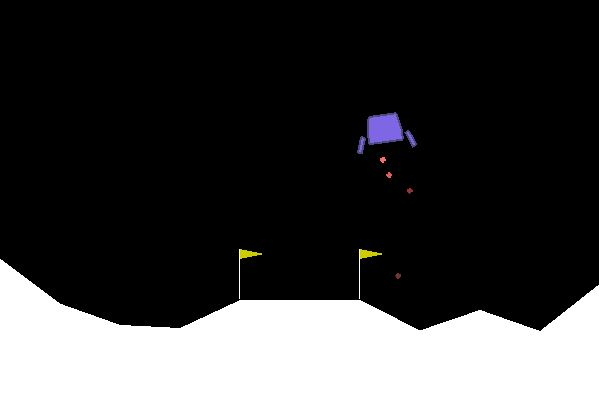
\includegraphics[width=0.7\textwidth]{lunar_lander/lunar_lander_example_image.JPG}
    \caption{OpenAi Gym's \glqq LunarLander-v2\grqq{}} \label{img:lunarLanderExample}
\end{figure}

Zu Beginn jeder Episode spawnt der Lander am oberen Bildschirmrand mit einem zufälligen Winkel und einer leicht variierenden Position. Sein Zustand wird mit sieben Attribute beschrieben: Die horizontale und vertikale Koordinate, die horizontale und vertikale Geschwindigkeit, der Winkel und die Winkelgeschwindikeit der Kapsel und ob die einzelnen Landefüße (2 Stück) den Boden berühren. Die Belohnung hängt von mehreren Komponenten ab: Ob sich der Lander der Landezone nähert oder sich davon entfernt, ob er zum Stillstand kommt oder crasht, ob seine Füße den Boden berühren und natürlich ob er sich in der Landezone befindet. Außerdem erhält er eine kleine Strafe jedes Mal, wenn er das Haupttriebwerk benutzt. Dies ist neben nichts tun, linkes Triebwerk benutzen und rechtes Triebwerk benutzen eine der vier möglichen Aktionen.

Der in diesem Kapitel verwendete Lernalgorithmus ist bis auf kleine Anpassungen mit dem aus Kapitel \ref{sec:deepQImplementation} identisch. Der Hauptunterschied ist, dass dieses Mal ReLu als Activation-Function der Hidden-Layers verwendet wird.

\section{Experimente}
\paragraph{Klassisches $ \epsilon $-greedy}
Wir beginnen wieder mit dem klassischen $ \epsilon $-greedy Ansatz. Nach einigen Vorabtests wählen wir die Hyperparameter wie folgt:
\begin{minted}{python}
params = DeepQParameters(
            num_episodes=2500,
            max_steps_per_episode=0,
            replay_buffer_size=20000,
            batch_size=32,
            learning_rate=0.001,
            discount_rate=0.99,
            target_update=10,
            start_exploration_rate=1,
            max_exploration_rate=1,
            min_exploration_rate=0,
            exploration_decay_rate=0.005,
            # ... Rest wird erst während des Trainings belegt
        )
\end{minted}
Hierbei fällt auf, dass die \mintinline{python}{max_steps_per_episode} auf \mintinline{python}{0} gesetzt sind. Dies liegt daran, dass eine Episode endet, sobald der Lander das Bild verlässt, crasht oder zum Stillstand kommt. Aufgrund der sehr langen Trainingszeit beschränken wir die Anzahl der Iterationen pro Experiment auf 10.

\begin{figure}[h!]
    \centering
    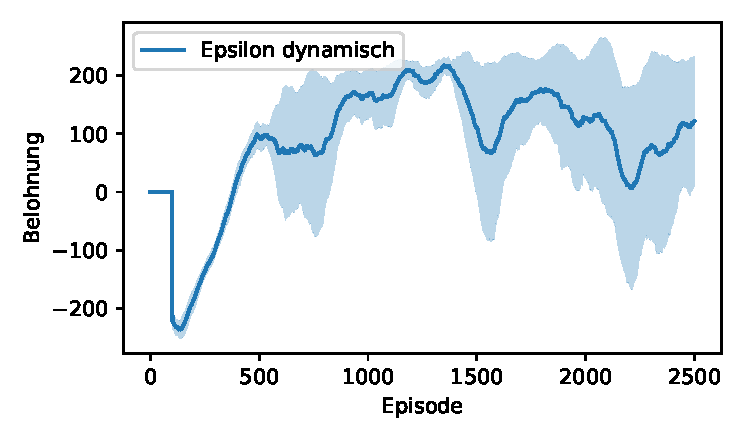
\includegraphics[width=0.7\textwidth]{lunar_lander/figure_classic_epsilon_03.pdf}
    \caption{TODO} \label{img:graphClassicEps01}
\end{figure}

Der Graph \ref{img:graphClassicEps01} zeigt wieder den durchschnittlichen moving average mitsamt seiner Standardabweichung. Die Kurve steigt bis Episode 500 stetig an. Ab hier wird der Agent allerdings sehr inkonsistent. Der Durchschnitt pendelt sich nicht bei einem Wert ein, sondern fluktuiert stark. Auch die Standardabweichung bricht stark aus. Die einzelnen Ergebnisse variieren ebenfalls sehr stark. Im ersten Durchlauf hat der Agent gelernt, die Kapsel sehr sanft direkt auf der Landeplattform zu landen. Im zweiten Durchlauf scheint der Agent keinen merklichen Lernfortschritt gemacht zu haben, da er bei jedem Landeanflug sofort crasht.

\paragraph{Vergleich der unterschiedlichen Ansätze}
Trotz des unbefriedigenden Resultats des vorherigen Experiments werden wir dieses mit den anderen Ansätzen vergleichen. Wir führen zu diesem Zweck ein Experiment ohne Erkundungsstrategie und eines mit modifizierter Belohnung durch. 

% Der Graph \ref{img:graphClassicEps01} zeigt wieder den durchschnittlichen moving average mitsamt seiner Standardabweichung. Der Agent scheint bis Episode 1000 einen sehr ordentlichen Lernfortschritt zu machen. Die Lernkurve beginnt hier steil und flacht dann langsam ab, so wie es wünschenswert ist. Nach Epsiode 1000 fällt die Kurve allerdings nochmals stark ab und die Standardabweichung bricht stark aus. Kurz darauf steigt der Wert wieder und erreicht ein neues Maximum, bevor er wieder leicht abfällt. Der Agent landet den Lander bei der Anwendung des DQNs relativ ruppig und lässt nach der Landung meist die seitlichen Triebwerke laufen.

% Da dieses Verhalten noch nicht optimal ist und der Graph gegen Ende ziemlich kurvig wird, führen wir das Experiment nochmals mit 2500 Episoden durch. Da eine Iteration dieses Experiments deutlich länger dauert als beim Navigations-Problem, setzen wir die Wiederholungen pro Experiment auf 10 herab, um die Versuche in absehbarer Zeit durchführen zu können.

% \begin{figure}[h!]
%     \centering
%     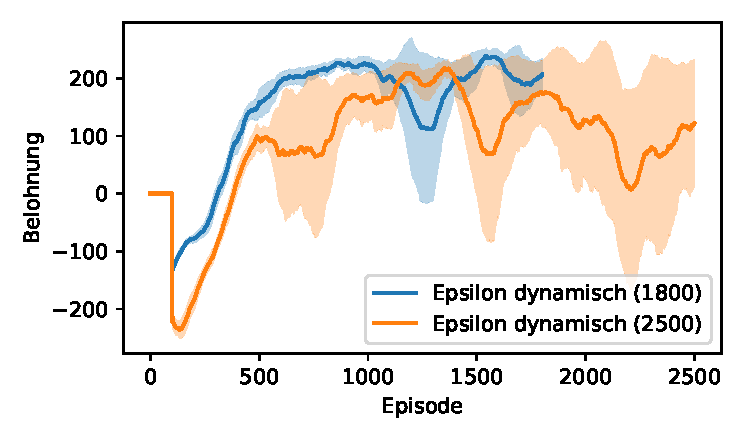
\includegraphics[width=0.7\textwidth]{lunar_lander/figure_classic_epsilon_02.pdf}
%     \caption{TODO} \label{img:graphClassicEps02}
% \end{figure}

% In Graph \ref{img:graphClassicEps02} ist zu sehen, dass das neue Experiment (orange) trotz (bis auf die Episodenanzahl) identischer Parameter etwas anders verläuft als das letzte. Der Belohnungsdurchschnitt erreicht etwa dort seinen Höhepunkt, wo der vorangegangene Versuch nochmals eingebrochen ist und umgekehrt. Wir vermuten, dass dies an der sensiblen Umgebung liegen kann. Eine kleine Aktion hat hier eine relativ große Auswirkung. So kann beispielsweise das Zünden eines der Steuertriebwerke im falschen Moment zum Kippen des Landers und somit zum Crash führen.

% Nichtsdestotrotz zeigen einige Stichproben mit den gelernten DQNs, dass der Agent durchaus meistens nach dem Training dazu in der Lage ist, das Raumschiff sehr sanft und zielgenau zu landen. Dies wird wahrscheinlich dadurch ermöglicht, dass wir auch hier am Ende das Netz ausgeben, welches während des Trainings den höchsten moving average produziert hat.

% TODO Boxplots












% \section{Experimente}
% \paragraph{Klassisches $ \epsilon $-greedy}
% Wir beginnen wieder mit dem klassischen $ \epsilon $-greedy Ansatz. Außerdem ist die Episodenanzahl aus dem gleichen Grund verhältnismäßig gering gewählt. Nach einigen Vorabtests haben sich die folgenden Hyperparameter herauskristallisiert:
% \begin{minted}{python}
% params = DeepQParameters(
%             num_episodes=1800,
%             max_steps_per_episode=0,
%             replay_buffer_size=20000,
%             batch_size=32,
%             learning_rate=0.001,
%             discount_rate=0.99,
%             target_update=10,
%             start_exploration_rate=1,
%             max_exploration_rate=1,
%             min_exploration_rate=0,
%             exploration_decay_rate=0.005,
%             # ... Rest wird erst während des Trainings belegt
%         )
% \end{minted}
% Hierbei fällt auf, dass die \mintinline{python}{max_steps_per_episode} auf \mintinline{python}{0} gesetzt sind. Dies liegt daran, dass eine Episode endet, sobald der Lander das Bild verlässt, crasht oder zum Stillstand kommt.

% \begin{figure}[h!]
%     \centering
%     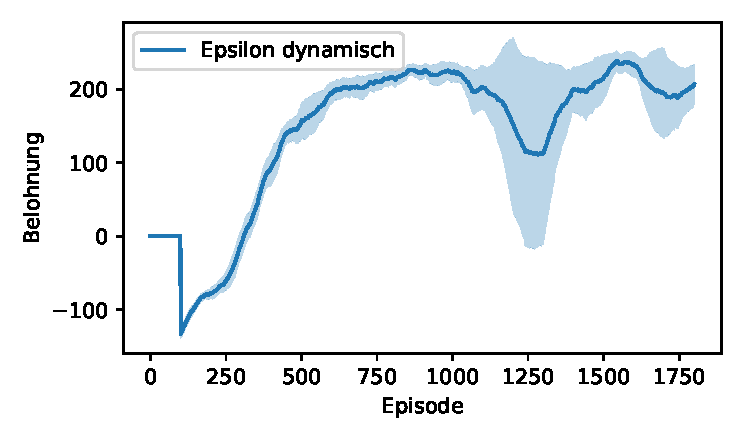
\includegraphics[width=0.7\textwidth]{lunar_lander/figure_classic_epsilon_01.pdf}
%     \caption{TODO} \label{img:graphClassicEps01}
% \end{figure}

% Der Graph \ref{img:graphClassicEps01} zeigt wieder den durchschnittlichen moving average mitsamt seiner Standardabweichung. Der Agent scheint bis Episode 1000 einen sehr ordentlichen Lernfortschritt zu machen. Die Lernkurve beginnt hier steil und flacht dann langsam ab, so wie es wünschenswert ist. Nach Epsiode 1000 fällt die Kurve allerdings nochmals stark ab und die Standardabweichung bricht stark aus. Kurz darauf steigt der Wert wieder und erreicht ein neues Maximum, bevor er wieder leicht abfällt. Der Agent landet den Lander bei der Anwendung des DQNs relativ ruppig und lässt nach der Landung meist die seitlichen Triebwerke laufen.

% Da dieses Verhalten noch nicht optimal ist und der Graph gegen Ende ziemlich kurvig wird, führen wir das Experiment nochmals mit 2500 Episoden durch. Da eine Iteration dieses Experiments deutlich länger dauert als beim Navigations-Problem, setzen wir die Wiederholungen pro Experiment auf 10 herab, um die Versuche in absehbarer Zeit durchführen zu können.

% \begin{figure}[h!]
%     \centering
%     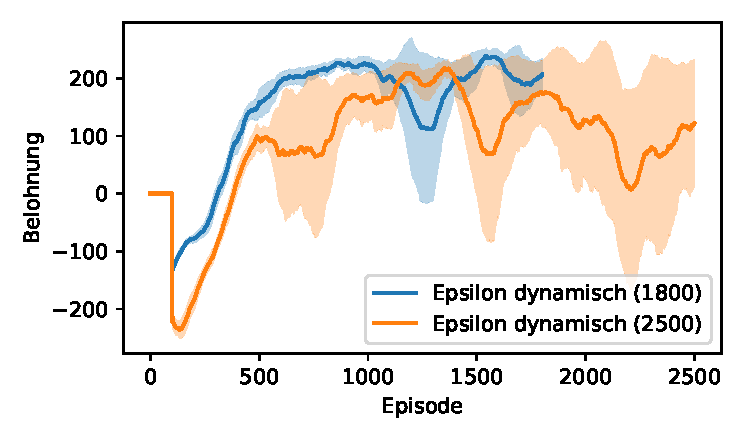
\includegraphics[width=0.7\textwidth]{lunar_lander/figure_classic_epsilon_02.pdf}
%     \caption{TODO} \label{img:graphClassicEps02}
% \end{figure}

% In Graph \ref{img:graphClassicEps02} ist zu sehen, dass das neue Experiment (orange) trotz (bis auf die Episodenanzahl) identischer Parameter etwas anders verläuft als das letzte. Der Belohnungsdurchschnitt erreicht etwa dort seinen Höhepunkt, wo der vorangegangene Versuch nochmals eingebrochen ist und umgekehrt. Wir vermuten, dass dies an der sensiblen Umgebung liegen kann. Eine kleine Aktion hat hier eine relativ große Auswirkung. So kann beispielsweise das Zünden eines der Steuertriebwerke im falschen Moment zum Kippen des Landers und somit zum Crash führen.

% Nichtsdestotrotz zeigen einige Stichproben mit den gelernten DQNs, dass der Agent durchaus meistens nach dem Training dazu in der Lage ist, das Raumschiff sehr sanft und zielgenau zu landen. Dies wird wahrscheinlich dadurch ermöglicht, dass wir auch hier am Ende das Netz ausgeben, welches während des Trainings den höchsten moving average produziert hat.

% TODO Boxplots